\chapter{Introdução}    %3° pessoa  %Verbos no passado      %Max de trés páginas
    \label{chp:introducao}
    \section{Definição do problema e motivação}
        %Contextualização
        Um robô industrial é um sistema robótico usado para manufatura, sendo que sua utilização contribui para o aumento da flexibilidade de sua célula de produção, de forma semelhante às máquinas \ac{CNC}. Assim, caso o objeto a ser produzido seja atualizado ou mesmo trocado por um novo modelo, geralmente demanda uma mudança na programação e, as vezes, da ferramenta. Já as máquinas dedicadas a uma tarefa específica de fabricação são mais rígidas e difíceis de serem adaptadas a mudanças no produto. É bem verdade que máquinas específicas geralmente apresentam maior volume de produção. De acordo com a \ac{ISO}, um robô industrial é definido como "um manipulador controlado automaticamente, reprogramável, multifuncional, programável em três ou mais eixos, que pode ser fixo ou móvel para uso em aplicações de automação industrial".
        
        Existem algumas formas de classificação de robôs, segundo seu número e tipo de juntas, por exemplo, que podem ser rotacionais (R) ou prismáticas (P). Assim, tem-se os robôs cartesianos, que são PPP, ou os robôs cilíndricos (RPP), os esféricos (RRP) e os antropomorfos (RRR). Outra classificação separa os robôs industriais em manipuladores de propósito geral e manipuladores de uso específico, como é mostrado na Figura~\ref{fig:tipos}. Um robô de propósito geral é basicamente um suporte de ferramentas articulado e programável, capaz de movimentar e posicionar a ferramenta que for fixada em sua extremidade (flange) com considerável precisão. Já um manipulador de uso específico, terá seu projeto otimizado para a realização de determinada tarefa, tendo uma ferramenta específica e cabos e mangueiras integradas a sua estrutura mecânica. Um exemplo de robô de uso específico é o de soldagem a arco~\cite{spong2005robot}.
        
        \begin{figure}[h]
            \centering
            \begin{subfigure}[b]{0.4\textwidth}
                \centering
                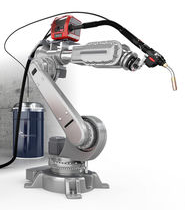
\includegraphics[width=6cm]{imagens/Fotos/Robo_de_proposito_geral.png}
                \caption{}
                \label{fig:robo_geral}
            \end{subfigure}
            \hfill
            \begin{subfigure}[b]{0.49\textwidth}
                \centering
                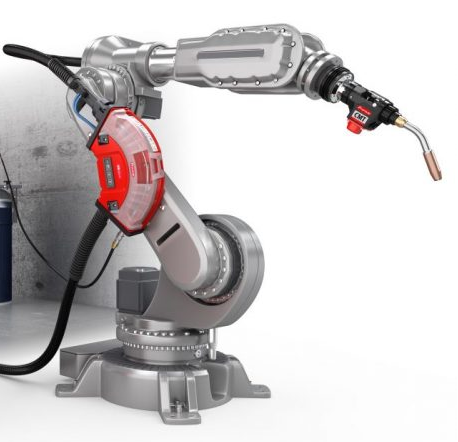
\includegraphics[width=7cm]{imagens/Fotos/Robo_dedicado.png}
                \caption{}
                \label{fig:robo_dedicado}
            \end{subfigure}
            \caption{Robô de propósito geral (a) e dedicado à soldagem (b)}
            \label{fig:tipos}
        \end{figure}
        
        Com relação às partes constituintes, um robô industrial é dividido em sua estrutura mecânica, na unidade controladora e no \ac{TP}. Podem integrar o sistema robótico diferentes ferramentas, dispositivos auxiliares, como trilhos para movimentação do robô, e dispositivos periféricos, como mesas móveis do tipo pórtico.  
        
        Os robôs industriais tradicionais possuem a unidade controladora uma arquitetura fechada de controle e geração de trajetória fornecida pelo fabricante. Esse tipo de solução segue o paradigma a qual deve ser priorizada a robustez e confiabilidade do funcionamento e da execução das tarefas, além de atender a certos requisitos normativos e legais que regem as indústrias. A controladora desses robôs é programada via uma linguagem dedicada, normalmente derivada de uma linguagem de programação de propósito geral acrescentada das funcionalidades necessárias aos robôs, como os comandos MOVE. Logo, cada fabricante de robô possui sua própria linguagem dedicada, os robôs ABB são programados na linguagem RAPID, os robôs Kuka em KRL, os robôs Comau em PDL2, etc. A linguagem PDL2 é derivada da linguagem PASCAL, por exemplo.
        
        Portanto, as controladoras fechadas buscam atender os requisitos de confiabilidade e também de simplicidade, demandando pouco conhecimento ou treinamento para operar ou programar um robô. No entanto, é perceptível que essa forma dificulta a realização de novas implementações e atividades de pesquisa com os robôs industriais. Ao mesmo tempo que estabelece, em certo ponto, uma dependência com os fabricantes e/ou com as empresas parceiras quando surge a necessidade de uma mudança ou expansão da célula de produção robotizada.
        
        Existem alguns fabricantes de robôs industriais, como a Comau, a Universal Robots, a Staubli e a Kuka, que possuem a opção de controladora aberta, isto é, controladoras que permitem programação utilizando linguagens de propósito geral, como C ou C++. A vantagem de usar esse tipo de linguagem, em comparação com o uso de uma linguagem dedicada à robótica, é que as possibilidades de uso são expandidas, por exemplo, é possível criar seu próprio gerador de trajetória, utilizar visão computacional para controlar a pose do robô, realizar um controle de força, substituir os controladores das juntas do robô, entre outras possibilidades. Isso vai mais ao encontro às novas demandas da Industria 4.0, bem como dos pesquisadores e desenvolvedores. Por exemplo, se surge a demanda por acrescentar uma malha de controle com visão computacional, poder-se-a integrar uma ou mais câmeras que tenham um bom custo, e não câmeras de um fornecedor específico, que geralmente apresentam custo mais elevado.  
        
        %DESVANTAGENS: Porque a maioria dos fabricantes de robôs industriais não possuem a opção de controladoras abertas?
        %(esta é uma das tais perguntas chave, no sentido de que vale a pena abordar e tentar responder)
        O paradigma de controladora aberta não atende todos os interesses das industrias, por exemplo, a industria demanda que a programação do equipamento seja facilmente aprendida por pessoas com baixa qualificação profissional e uma linguagem dedicada à robótica é concebida justamente com essa intenção, o que não é o caso do C e C++, já que, por serem de propósito geral, possuem muito mais funcionalidades do que apenas mover o robô por uma trajetória. Além disso, como comentado anteriormente, o paradigma da controladora fechada oferece mais robustez e confiabilidade de seu funcionamento e da execução das tarefas. 
        
        A Comau desenvolveu uma controladora aberta que é uma variante de sua controladora padrão. A abertura é realizada mediante a adição de um pequeno hardware de comunicação e um software ao PLC da controladora com objetivo de implementar a comunicação com um computador industrial fornecido pela fabricante. Neste computador são executado os programas desenvolvidos pelo usuário em C ou C++ com a possibilidade de controlar a posição, velocidade ou torque das juntas do robô, ao mesmo tempo que lê os dados sensoriais do robô. Dessa forma, a controladora aberta continua trabalhando da mesma forma que a controladora fechada, com a exceção de quando é ativada a modalidade aberta pela aplicação do usuário em sua linguagem dedicada, a PDL2, que está em execução na mesma. Quando isso acontece, a aplicação do usuário no computador industrial passa a comandar o robô. Logo, a solução da Comau pode ser considerada uma solução híbrida, permitindo ao usuário alternar entre usar a linguagem robótica para controlar o robô, ou usar a linguagem C/C++ para controlar o mesmo através da sua implementação.
        
        %Problema
        Apesar dessa solução inovadora, ela possui certas limitações, por exemplo, a linguagem de programação do desenvolvimento das aplicações é restrita à linguagem C ou C++, ao hardware fornecido pelo fabricante (o computador industrial) tanto em relação a potência computacional quanto à arquitetura do mesmo, ficando restrito também ao sistema operacional fornecido pelo fabricante.
        
        %Justificativa / Motivação
        Assim sendo, pareceu relevante a tentativa de se investigar se seria possível dar mais liberdade no desenvolvimento de aplicações para um robô industrial com controladora aberta, onde um terceiro dispositivo ficaria responsável por realizar todo o processamento necessário para a geração de trajetória e enviar essa referência de posição ao computador industrial fornecido pela fabricante do robô, que por sua vez repassaria a referência para a controladora do robô. Assim, tal computador industrial ficaria responsável por receber as referências e repassar para a controladora do robô.
        
        %Tema
        A proposta deste trabalho de conclusão de curso é desenvolver um arranjo cliente servidor para o computador industrial que possibilitará o desenvolvimento de aplicações em qualquer linguagem de programação, qualquer arquitetura e qualquer sistema operacional para um terceiro dispositivo que seja capaz de se conectar com o mesmo pelo protocolo \ac{TCPIP}, sendo o arranjo cliente servidor responsável apenas por ser uma ponte de comunicação entre a controladora do robô e o software rodando no terceiro dispositivo. Assim, dando mais liberdade aos desenvolvedores de aplicações para a Industria 4.0 e para os pesquisadores universitários, atendendo inclusive a demanda do Laboratório de Robótica do CEFET-MG, o qual possui uma controladora desse tipo, a C5G Open, disponível.
        
        %Colocar foto do robô e da controladora
        %\begin{figure}[!htb] 
        %    \centering
        %    \includegraphics[width=13cm]{Imagens/}%\columnwidth
        %    \small
        %    \centering
        %    \caption{Vista do sistema robótico no laboratório}
        %    \label{fig:introducao}
        %\end{figure}

	    %Hipótese
	    Parte-se da hipótese de que seja possível desenvolver um software que se comunique com a controladora do robô via protocolo fornecido pela fabricante ao mesmo tempo, porém em taxas diferentes, que se comunica com um software em um terceiro dispositivo via protocolo \ac{TCPIP}, sendo este terceiro dispositivo rodando um sistema operacional diferente, com uma arquitetura diferente e tal software em uma linguagem de programação diferente da exigida pela solução da fabricante. Assim, para viabilizar o teste dessa hipótese, realiza-se uma pesquisa de finalidade aplicada, objetivo exploratório, sob o método hipotético-dedutivo, com abordagem quantitativa, realizada com procedimentos experimentais. %Metodologia
        
    \section{Objetivos} %Objetivo geral     %Objetivos Específicos
        O objetivo geral do trabalho é desenvolver um software com arranjo do tipo cliente servidor, que estenda a liberdade que a solução de controladora aberta que a fabricante proporciona aos programadores de robôs industriais.
		
		\subsection{Objetivos específicos}
		    Para atingir o objetivo geral, é necessário desenvolver:
            \begin{itemize}
                \item Um protocolo de comunicação \ac{TCPIP} para enviar e receber variáveis referentes aos ângulos de juntas do robô.
                \item Uma função que salve na memória os ângulos de referência das juntas do robô oriundo do software no terceiro dispositivo, e que enviar os dados sensoriais armazenados na memória para tal software.
                \item Uma função use a solução da fabricante para ler dados sensoriais os salvando na memória e enviar referências das juntas do robô armazenadas na memória.
                \item E resolver o problema gerado pelo assincronismo da comunicação entre arranjo e controladora com o arranjo e o software no terceiro dispositivo.
            \end{itemize}
            
	\section{Organização do texto}  %Previa dos capítulos        %Hipótese        %Previa conclusão
	    
	    O Capítulo \ref{chp:Fundamentos} apresenta a revisão teórica do tema e assuntos tratados.  %apresenta o referencial teórico do tema e a referência bibliográfica dos assuntos tratados.
	    
	    O Capítulo \ref{chp:Desenvolvimento} apresenta o desenvolvimento do software arranjo cliente servidor e de um software cliente exemplo para realizar os testes e coletar os resultados experimentais.
	    
	    Já o Capítulo \ref{chp:Resultados} apresenta os resultados experimentais e discute a consequência deles.
	    
	    Ao final deste trabalho conclui-se no Capítulo \ref{chp:Conclusão} que o objetivo de estender a liberdade que a solução da fabricante proporciona aos programadores de robôs industriais foi atingido.
